\chapter{Dataset}
In total, two datasets were created, one for the detection of dental caries and the other for semantic segmentation of dental restorations. The majority of work was done on the former.

\begin{figure}
    \centering
    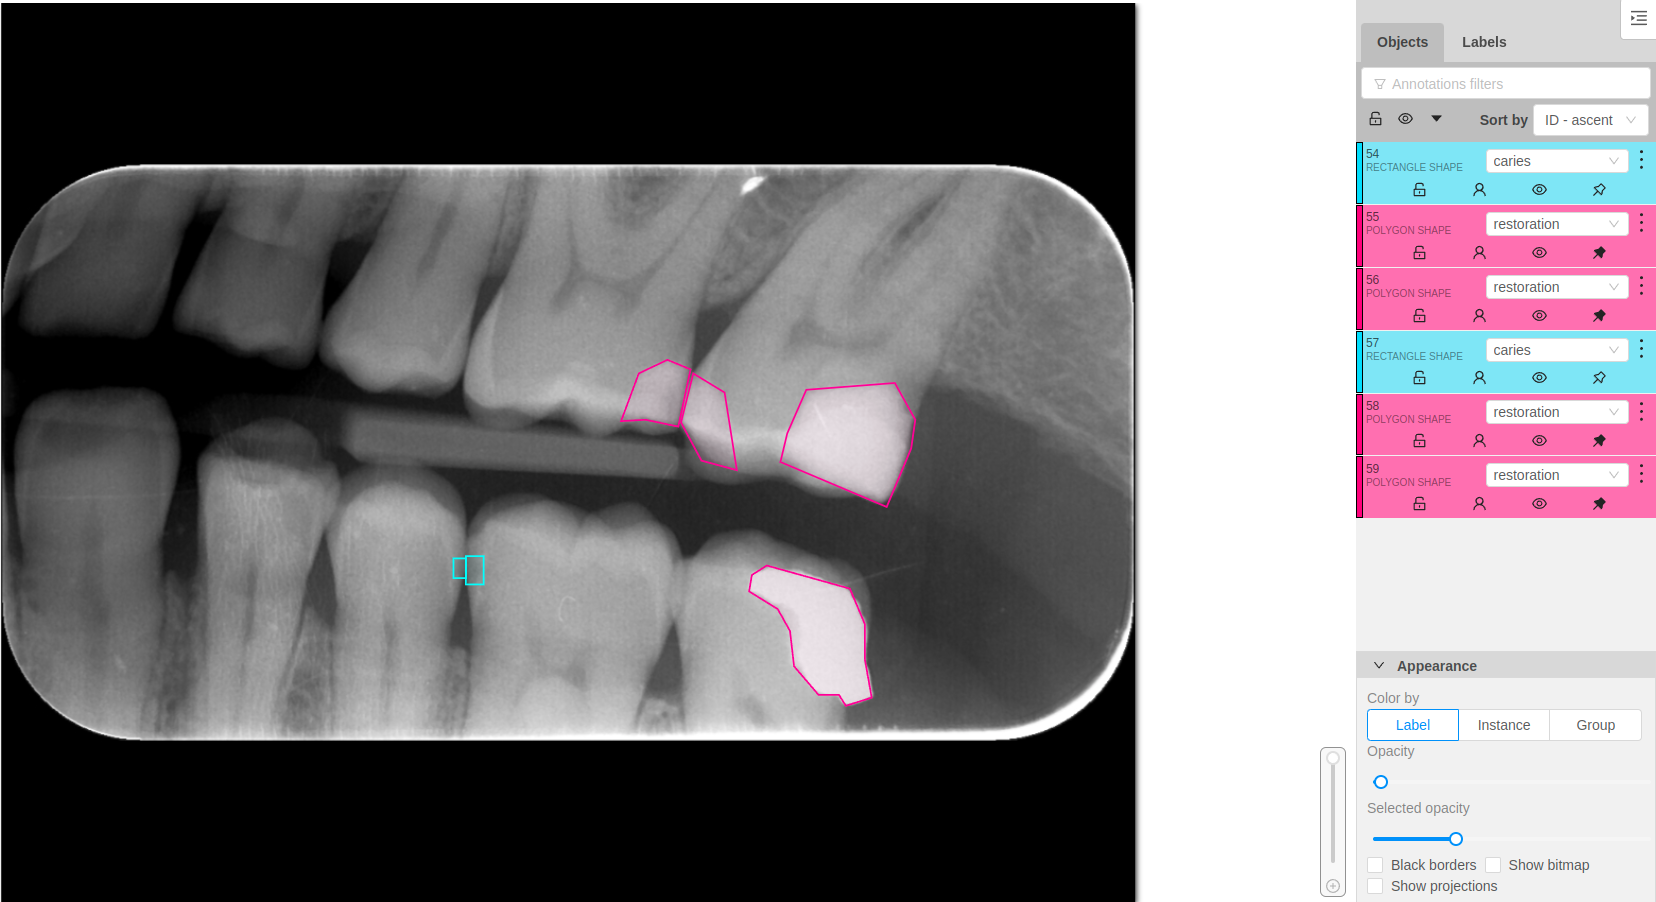
\includegraphics[width=\linewidth]{images/cvat.png}
    \caption{The evironment of CVAT with annotated carious lesion and dental restorations}
    \label{fig:cvat}
\end{figure}

\section{Dental caries}
The dataset was created by MDDr. Tichy and his team. The work on the dataset began in September of 2021, together with work on this thesis, and we were thus able to discuss the format of the data. We decided to annotate every dental caries lesion with a minimal bounding box. The annotation process was conducted in the Computer Vision Annotation Tool (CVAT), which was running on the Faculty of biomedical informatics server. The web address is www.gdiag.fbmi.cvut.cz.

While denoting the position of the carious lesion, the annotator tried to be consistent with the following guidelines:

\begin{itemize}
    \item Carious lesion is denoted by a rectangle. The whole lesion should lie inside the rectangle. The rectangle should be as tight as possible around the lesion.
    \item When the lesion is on the proximal surface, and booth teeth are infected, draw a separate box for each of them.
\end{itemize}

Due to constant work on the dataset, we decided to use the same data as long as there was no major update. This ensured that we could compare the performance of our models to each other until a major update was released. In total, six major releases were done. We call these releases stages of the dataset.

\subsubsection{First stage}
In the first stage MDDr. Tichy instructed a group of students of general dentistry on how to approach the annotation to get as homogenous a dataset as possible. Then they annotated a couple of images under his supervision before continuing on their own.
Dental X-ray images were uploaded into CVAT and divided into multiple projects, where each project contained between 400-800 images. This was done due to technical limitations regarding exporting and uploading X-ray images from a dental database. Each project was further split into jobs, each of them consisting of 100 images and assigned to a particular student. We had 1695 X-ray images at our disposal with 2416 dental caries annotated when the first stage was done. CVAT does not allow to export and merge of multiple tasks, so each task was exported separately in COCO format. All tasks were uploaded to the CMP server and merged together in one annotation.json file, which contained the information about the dataset in COCO format and file images, where we merged images from all annotated tasks. We checked the task for duplicate radiation and removed the. Furthermore, we removed any X-rays that were not yet reviewed. This resulted in 1626 images with 2399 decay annotations. From those, only 946 images contained at least one cavity.


\subsubsection{Second stage}
After inspection of the dataset created in the first stage, we observed in-homogeneity across annotations. Some of the guidelines were violated, especially the error-prone annotation of caries on proximal surfaces. In addition, multiple overlooked lesions were observed. This led us to reconsideration of our approach to labeling, and MDDr Tichy himself did all the annotation work from this moment further on. After the second stage, the dataset was extended to 2599 non-duplicate images containing 4328 annotations of tooth decay. In this stage, no corrections of previous errors were done.

\subsubsection{Third stage}
MDDr Tichy reviewed all images annotated in the first stage. An unspecified amount of annotations was removed as well as added. In the end, the dataset consisted of 2599 images with 4575 annotations of dental caries.

\subsubsection{Fourth stage}
Another 1400 images were uploaded onto the CVAT server. After training the model on the dataset created in stage three, the model achieved a performance of $AP@.5=0.61$. We downloaded all newly uploaded images and used the model to make predictions for those images. The confidence threshold achieving the best results on the validation dataset was used to filter out low-confidence predictions. We used the Voxel Fiftyone tool to upload all 1400 images and their respective predictions to CVAT, where those images were split into two separate tasks.
MDDr Tichy reviewed all predictions. Adjustments of bounding boxes as well as their removal and addition were conducted, according to personal statistics of MDDr. Tichy, there were roughly 200 predictions per 100 images. Around 20 predictions had to be added and removed in order to get the same quality annotations as in stage three. The upside of this approach was the speed, when annotation could be done in approximately half the time required to do the annotation without model predictions. In total, 3500 images were available after this stage. After removing corrupted images, we got 3489 images with 6087 annotations of carious lesions.

\subsubsection{Fifth stage}
In this stage, the annotation of all 1400 images uploaded in stage four was finished, resulting in 3989 X-rays with 7257 annotations.

\begin{table}
    \centering
    \begin{tabular}{l|r|r}
                                       & Width [px] & Height [px] \\\hline
        Image size                     & 1068       & 795-847     \\ \hline
        Minimal box size               & 8          & 9           \\ \hline
        Maximal box size               & 384        & 315         \\ \hline
        Mean of box size               & 47.55      & 53.15       \\ \hline
        Standard deviation of box size & 37.99      & 35.33       \\ \hline
    \end{tabular}
    \caption{\label{tab:dataset_statistics}Staticstcs of dental caries annotations in the dataset}
\end{table}

\subsubsection{Sixth stage}
We evaluated the performance of the model on the test, validation, and training part of the dataset. Although the model used for prediction achieved $AP@.5 = 0.72$, there were 1598 images with at least one false positive or false negative detection. We decided that doing a second round of dataset review would be more beneficial than further expansion of dataset size. We decided to focus only on erroneous images and uploaded 1598 images with at least a single error to the CVAT annotation tool for review.


\section{Dental restorations}
\begin{figure}
    \centering
    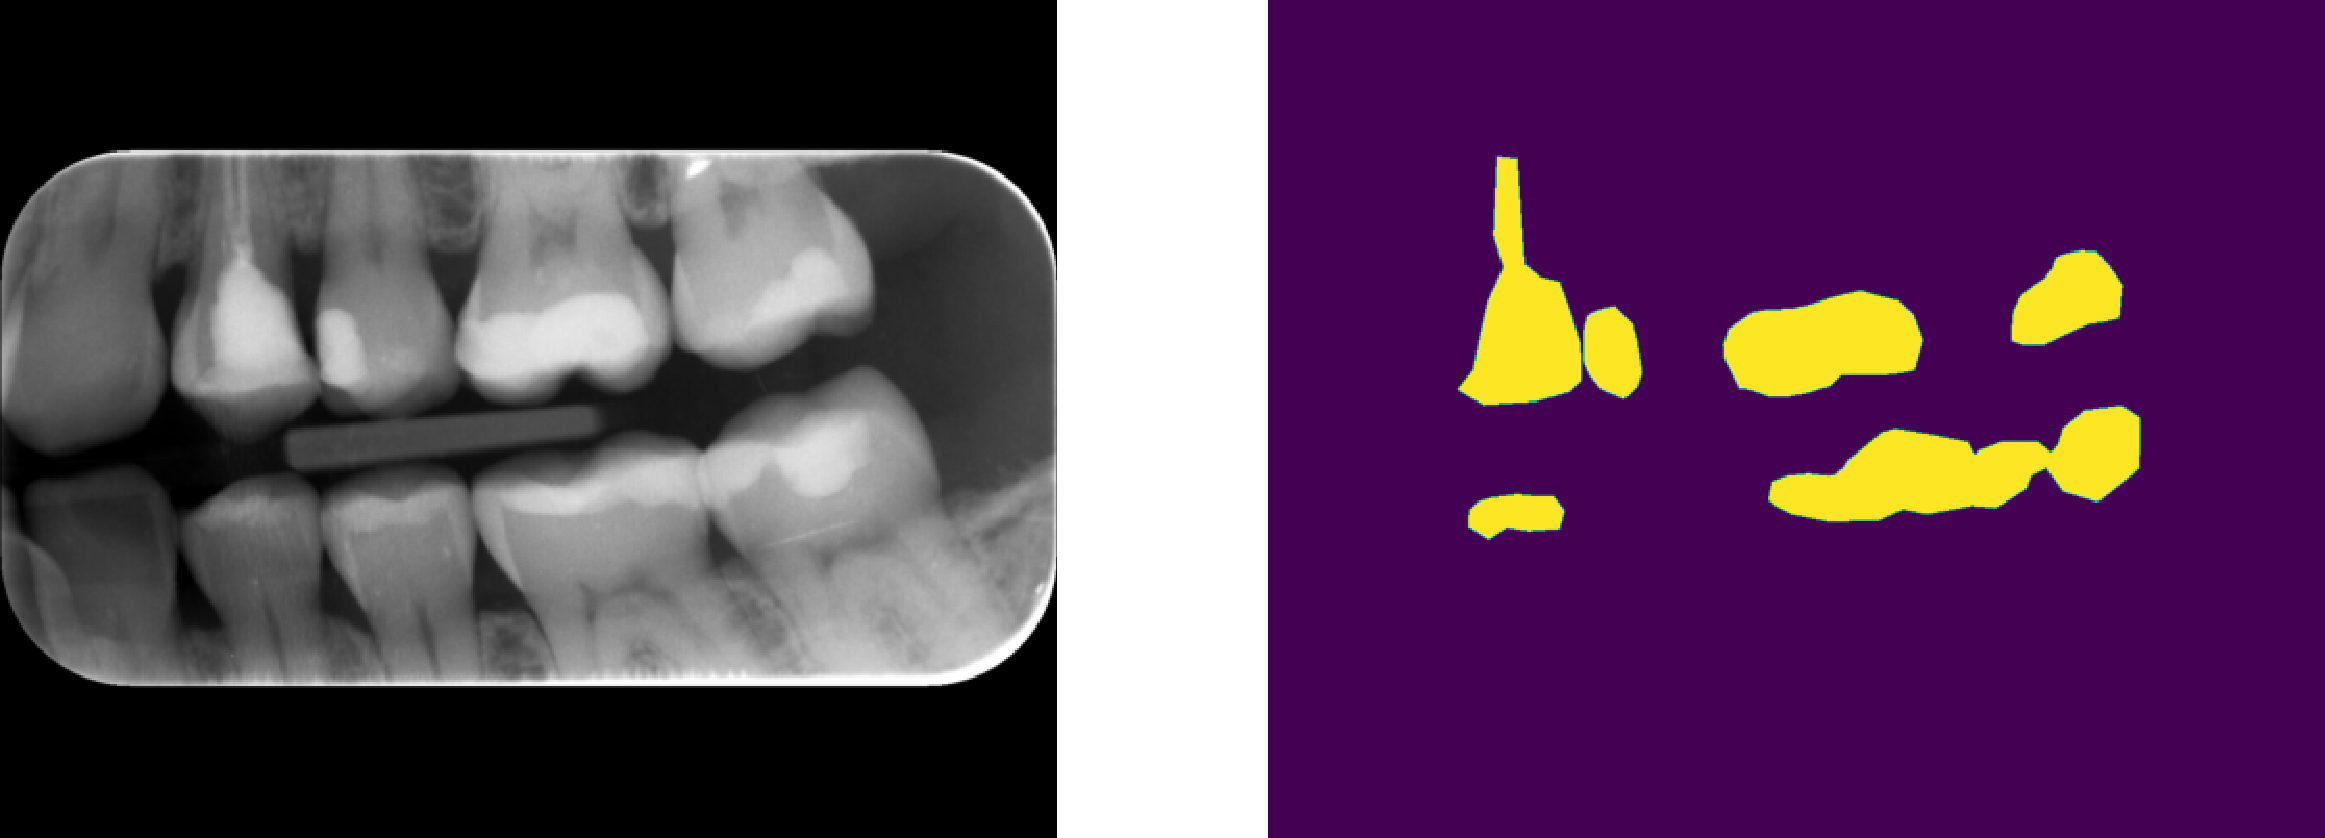
\includegraphics[width=\linewidth]{images/segmentation_ds_sample.pdf}
    \caption{Bitweing X-ray image on the left, pixel mask of the X-ray on the right (dental restorations have yellow color)}
    \label{fig:segmentation_sample}
\end{figure}
This dataset consists of a subset of images used in the dental caries dataset. It was annotated in the CVAT tool by drawing a polygon around each dental restoration. The work was done by the same group of dentistry students as stage one of the caries dataset and reviewed by a single fifth-year dentistry student. Checking the whole dataset by a single person should ensure consistency among images. A total of 521 images were used to create this dataset. Inspection of the dataset revealed that 387 radiographs contained at least a single annotated restoration, and 134 had none.
The dataset was exported from CVAT in COCO format and saved on the CMP server. When working with the data, we used a pixel mask instead of polygons to denote the position of dental restorations. A sample of the dataset with pixel mask can be seen in figure \ref{fig:segmentation_sample}.

In figure \ref{fig:segmentation_restoration_size} we can see, how many percent of X-ray image consists of restorations. This gives us an idea of how common restorations in our data are. In figure \ref{fig:segmentation_patch_size} we see, how size of individual restorations is distributed. Inspecting this figure, we observe that most restorations are smaller than $2\%$ of the image.

\begin{figure}
    \centering
    \begin{floatrow}[2]
        \ffigbox[\FBwidth]{\caption{Histogram of restoration area in image, images without restorations omited}\label{fig:segmentation_restoration_size}}%
        {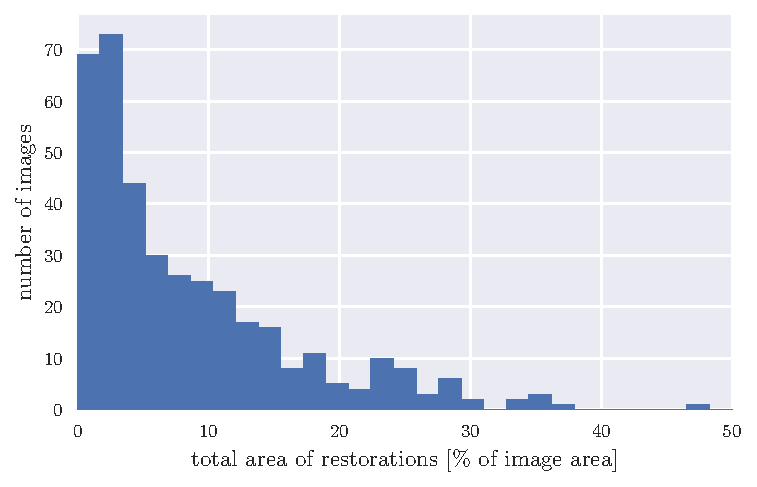
\includegraphics[width=\linewidth]{images/histogram_of_restoration_size.pdf}}\;
        \ffigbox[\FBwidth]{\caption{Histogram of areas of restorations, 10 largest omited}\label{fig:segmentation_patch_size}}
        {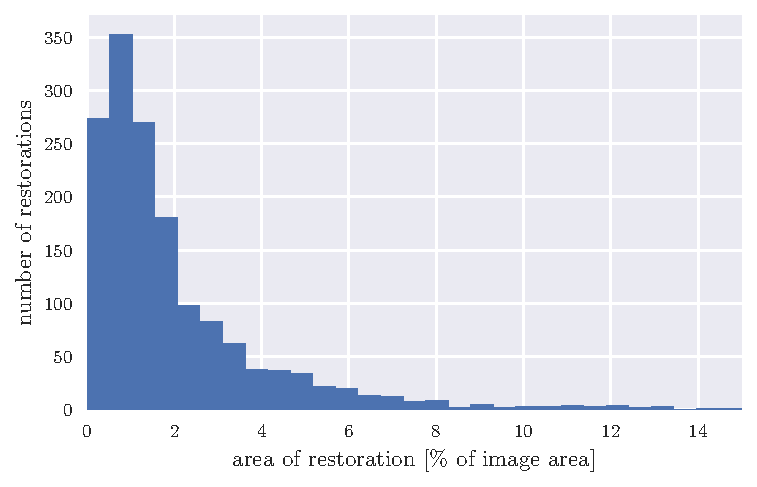
\includegraphics[width=\linewidth]{images/histogram_of_patch_size.pdf}}
    \end{floatrow}
\end{figure}